% !TEX root = ./AM3C.exercises_resolutions.2024.4.tex
\documentclass["AM3C.exercises_resolutions.2024.tex"]{subfiles}

% \tikzset{external/force remake=true} % - remake all

\begin{document}

\graphicspath{{\subfix{./.build/figures/AM3C.exercises_resolutions.2024.4}}}
% \tikzsetexternalprefix{./.build/figures/AM3C.exercises_resolutions.2024.4/graphics/}

\mymakesubfile{4}[AM3C]
{} % Subfile Title
{} % Part Title

\setcounter{question}{5}
\begin{questionBox}1{} % Q6
  Determine a deflexão \(u(x,t)\) da corda vibrante de comprimento \(L = \pi\), extremidades fixas, com \(c^2 = 1\) supondo uma velocidade inicial igual a zero e com uma deflexão inicial dada por \(f(x) = 0.01\,x\,(\pi − x)\).
  \answer{}
  \begin{flalign*}
    &
      u(x,0) = f(x) = 0.01\,x\,(\pi-x)
      % 
      % 
      % 
      ; &\\[3ex]&
      \odv[order=2]{u}{t}
      = c^2\,\odv[order=2]{u}{x}
      % 
      % 
      % 
      ; &\\[3ex]&
      u(x,t) = \sum_{h=1}^{+\infty}{A_h\,\sin(h\,x)\,\cos(h\,t)}
      % 
      % 
      % 
      ; &\\[3ex]&
      A_h
      = \frac{2}{\pi}
      \,\int_0^{\pi}{
        f(x)\,\sin(h\,x)
        \,\odif{x}
      }
      = \frac{2}{\pi}
      \,\int_0^{\pi}{
        (
          0.01\,x\,(\pi-x)
        )
        \,\sin(h\,x)
        \,\odif{x}
      }
      = &\\&
      = \frac{0.02}{\pi}
      \left(
        \pi
        \int_0^{\pi}{
          x
          \,\sin(h\,x)
          \,\odif{x}
        }
        -\int_0^{\pi}{
          x^2
          \,\sin(h\,x)
          \,\odif{x}
        }
      \right)
    &
  \end{flalign*}
  \begin{flalign}
    &
      \pi
      \int_0^{\pi}{
        x
        \,\sin(h\,x)
        \,\odif{x}
      }
      = \pi
      \left(
        -\frac{x}{h}
        \cos(h\,x)
        + \frac{1}{h^2}
        \,\sin(h\,x)
      \right)\Bigg\vert_{0}^{\pi}
      = \dots
      = (-1)^{h+1}\frac{\pi^2}{h}
      &\\[3ex]&
      -\int_0^{\pi}{
        x^2
        \,\sin(h\,x)
        \,\odif{x}
      }
      = \dots
      = - \left(
        -\frac{x^2}{h}\,\cos(h\,x)
        +\frac{2}{h^2}\,x\,\sin(h\,x)
        +\frac{2}{h^3}\,\cos(h\,x)
      \right)\Bigg\vert_0^\pi
      \notag
      = &\\&
      = - \left(
        \begin{matrix}
          -\frac{x^2}{h}\,\cos(h\,\pi)
          +\frac{2}{h^2}\,\pi\,\sin(h\,\pi)
          +\frac{2}{h^3}\,\cos(h\,\pi)
          \\
          -\frac{x^2}{h}\,\cos(h*0)
          +\frac{2}{h^2} *0*\sin(h*0)
          +\frac{2}{h^3}\,\cos(h*0)
        \end{matrix}
      \right)
      \notag
      = &\\&
      = - \left(
        (-1)^{n+1}
        \,\frac{\pi}{h}
        + \frac{2}{h^3}\left(
          (-1)^n-1
        \right)
      \right) 
      = \begin{cases}
        + \pi^2/h &\quad n\text{ par}
        \\
        -\pi^2/h + 4/h^3 &\quad n\text{ impar}
      \end{cases}
    &
  \end{flalign}
  \begin{center}
    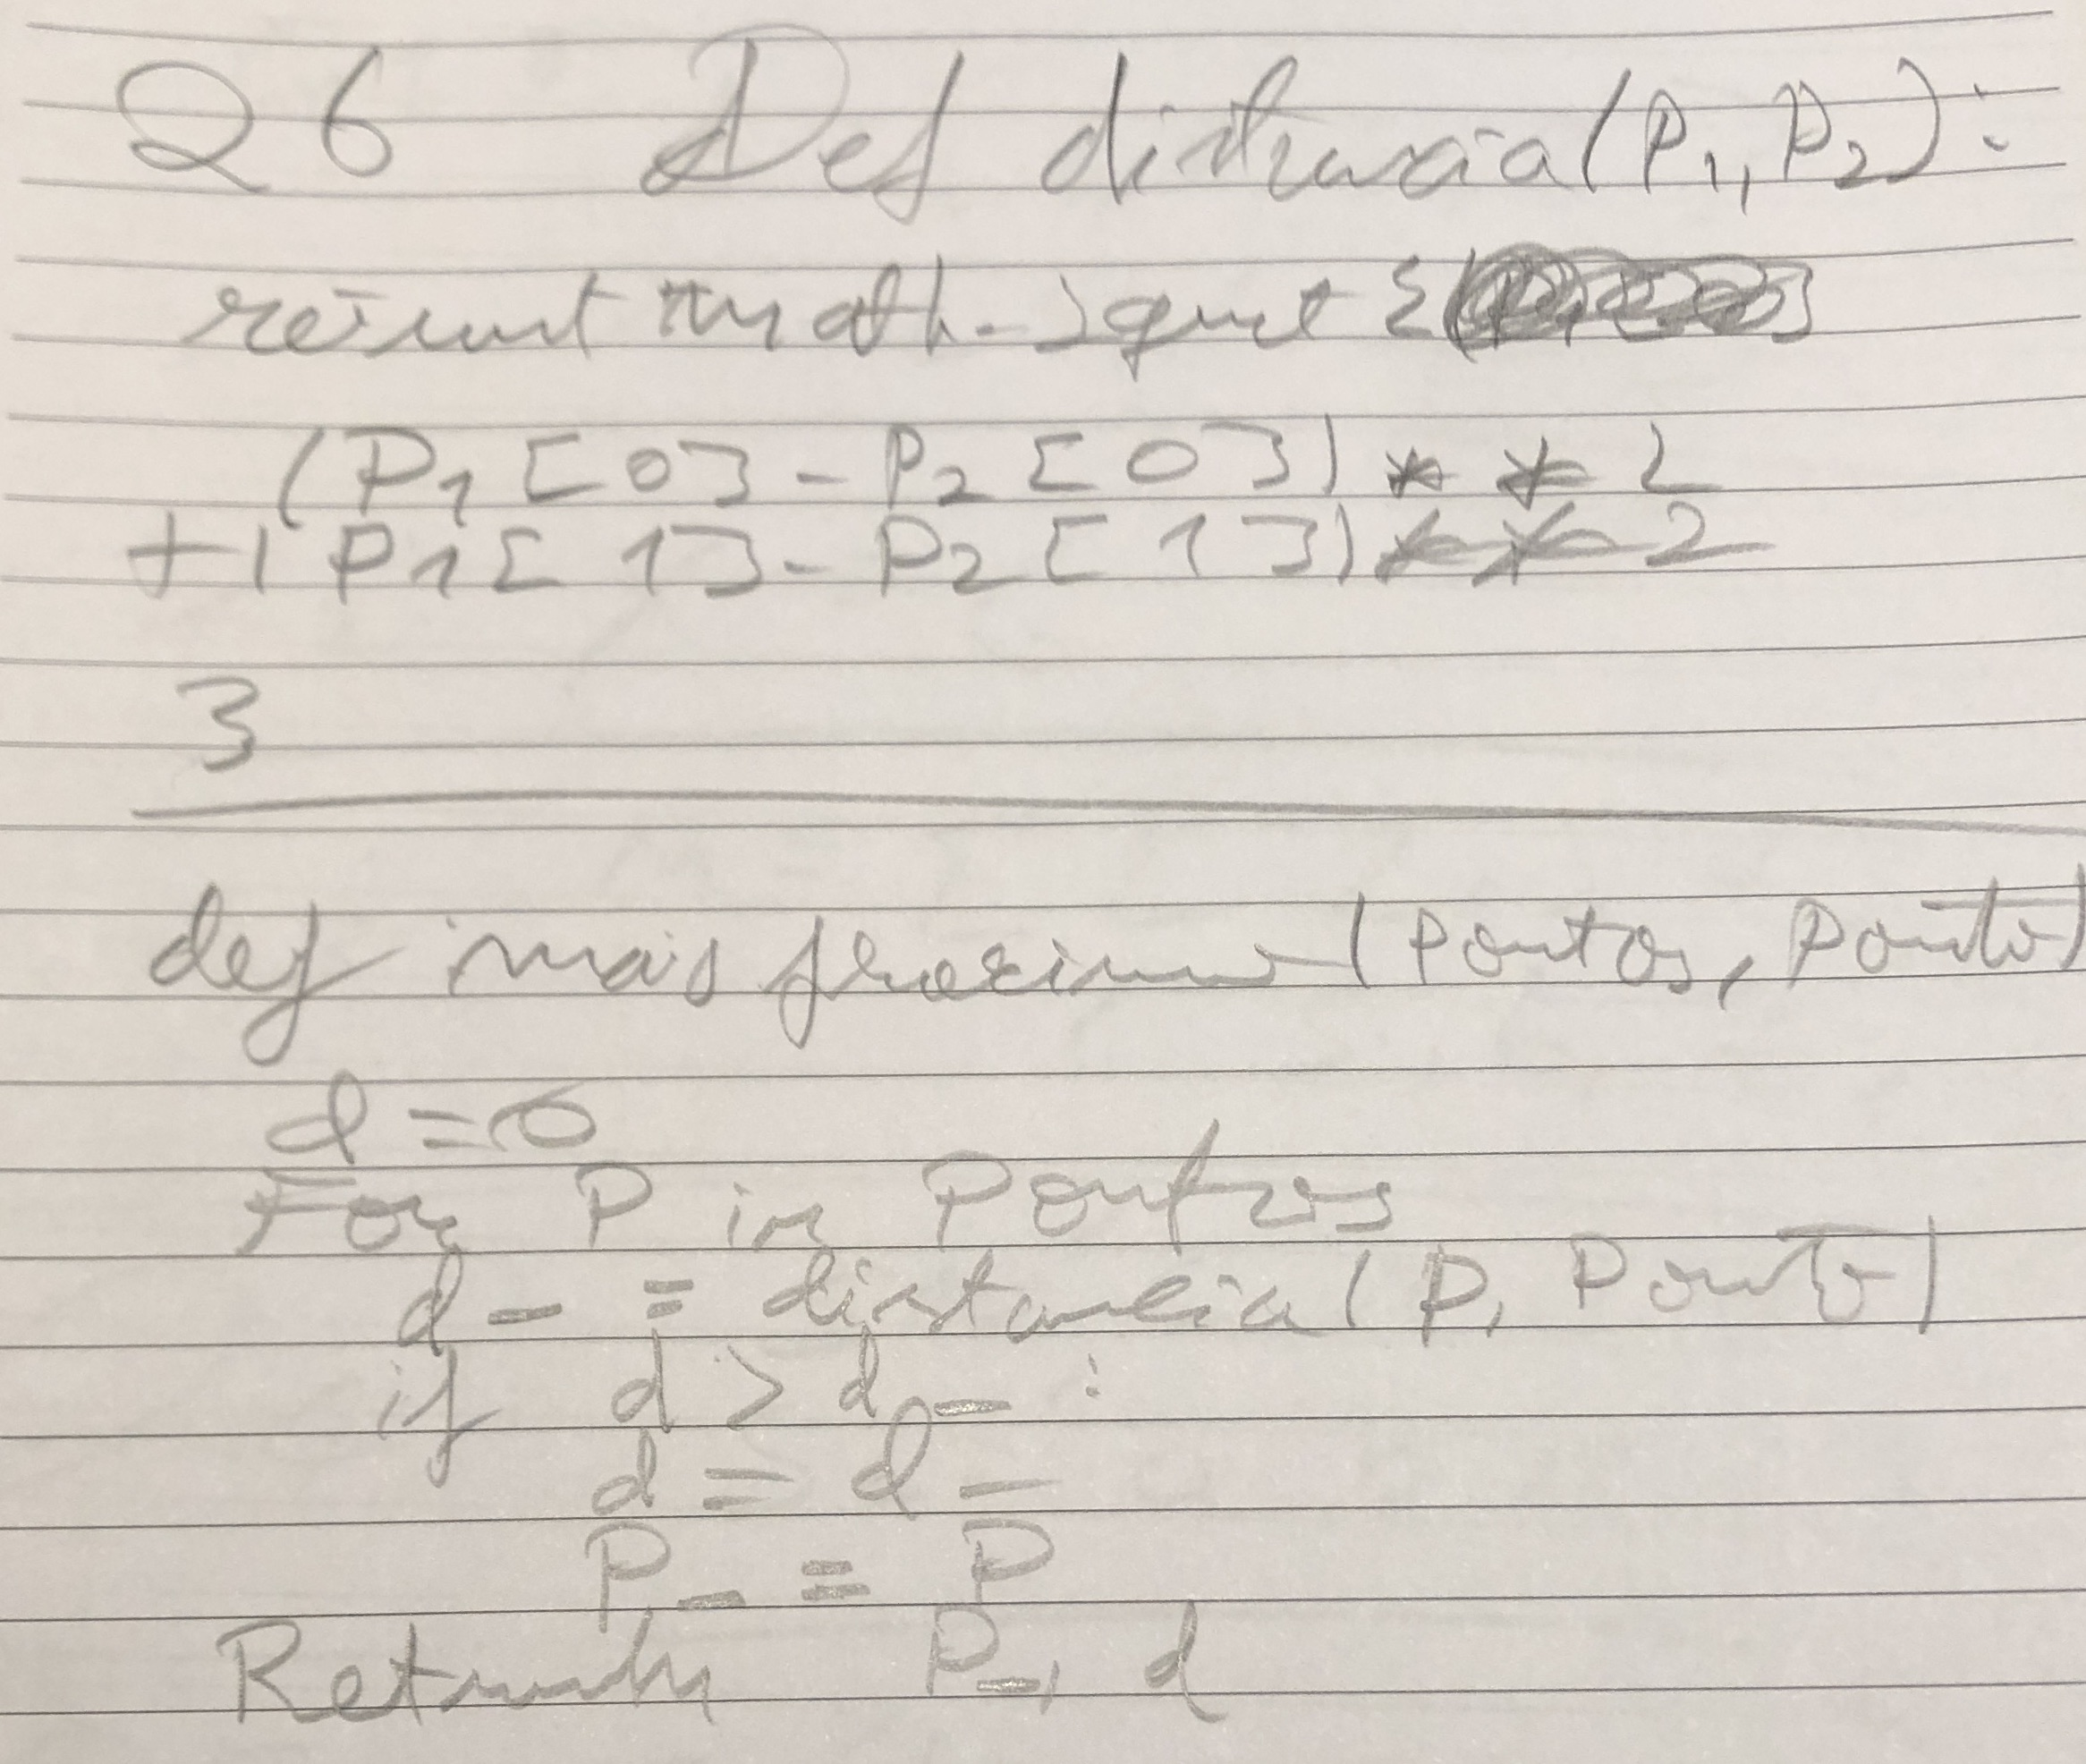
\includegraphics[width=.8\textwidth]{Q6.jpeg}
  \end{center}
\end{questionBox}

\end{document}
